
\chapter{Estado del arte y fundamentos teóricos}\label{estadoArte}

En este capítulo analizaré el estado actual del tema a tratar, junto con una pequeña revisión bibliográfica y algunos conceptos teóricos necesarios. Y profundizaré un poco más en las representaciones lineales comentadas en el Capítulo \ref{introduccion}, así como los distintos paquetes software existentes y sus limitaciones. 

\section{Revisión bibliográfica} \label{revision_bib}
Para el estudio de los trabajos relacionados y búsqueda de bibliografía se han consultado fuentes como IEEE Xplore, ACS Publications, o Journal of Chemical Information and Computer Sciences entre otras. En la Figura \ref{fig:revisionBibliografica} se exponen los resultados de un breve estudio bibliográfico sobre la literatura existente de los temas del proyecto. Todo comienza en 1988 con la publicación de David Weininger \cite{weininger_smiles_1988}, presentando SMILES como un nuevo formato de representación lineal, a partir de ahí y hasta día de hoy, fueron aumentando las publicaciones alrededor de SMILES. Sin embargo, vemos que apenas existe literatura para temas más específicos dentro de este área, como la canonización de las cadenas SMILES, o la organometálica. Los datos de las publicaciones se han recopilado a través de \textit{Scopus}\footnote{\url{https://www.elsevier.com/es-es/solutions/scopus}}\footnotecomma\footnote{\url{https://biblioteca.ugr.es/investigacion/herramientas-apoyo/evaluacion-publicaciones/scopus}} con las siguientes consultas, donde CHEM y COMP hacen referencia a chemistry y computer science respectivamente: 
\begin{itemize}
    \item {\footnotesize \textit{(SUBJAREA(CHEM) AND TITLE-ABS-KEY(smiles))}} 
    \item {\footnotesize \textit{((SUBJAREA(CHEM) OR SUBJAREA(COMP)) AND TITLE-ABS-KEY(smiles AND canonical))}}
    \item {\footnotesize \textit{(SUBJAREA(CHEM) AND TITLE-ABS-KEY(smiles AND organometallic))}}
\end{itemize}

\begin{figure}[h!]
        \centering
        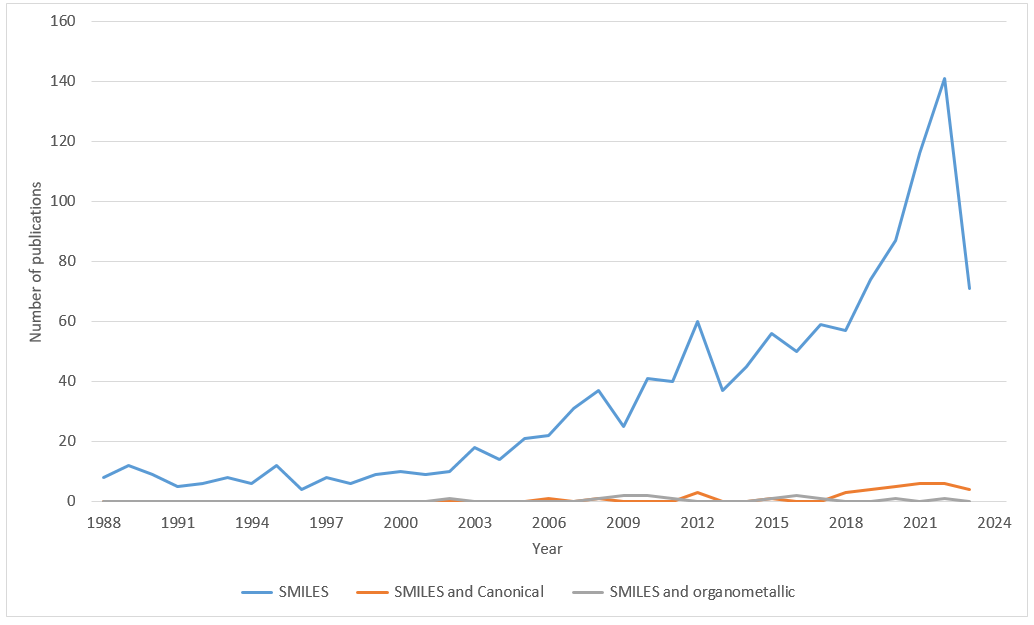
\includegraphics[scale=0.5]{imagenes/estado_arte/revisionBibliografica.png}
        \caption{Comparativa del número de artículos publicados por año según las palabras clave de la búsqueda. Imagen de elaboración propia. Datos extraídos de \emph{Scopus}.}
        \label{fig:revisionBibliografica}
    \end{figure}


\section{Fundamentos teóricos}

\subsection{Moléculas y sus representaciones}
representacion de moléculas (formula estructural conection tables, tipos de ficheros (.smi, .sdf, etc) representacion lineal y mas cosas),

\subsection{Representaciones lineales}
Hablar mas extendido de SMILES, SELFIES, e INCHI;

\subsection{Organometálica}
Cualquier concepto de quimica que me haga falta para entender el trabajo, o que haya tenido que aprender yo durante el mismo.
hablar de la regla de los 18 electrones y compuestos de coordinacion vs organometalicos
(mirar mashup)

\section{Herramientas o toolkits} \label{toolkits}

Existe una gran variedad de herramientas a la hora de trabajar dentro de la química computacional, tanto open-source como aplicaciones propietarias para las que son necesarias pagar una licencia de uso. La química computacional según comenté en el capítulo \ref{introduccion}, se aplica en muchos ámbitos de la ciencia. Como tal, hay herramientas con propósitos muy distintos: extensiones de navegador que mejoran el acceso a la información de las bases de datos \cite{safari_extensions}, cálculos de propiedades fisicoquímicas, cribado virtual de moléculas (ChemAxon, MOE, LigandScout, Forge), modelado y bocetado de moléculas (Marvin, ChemDraw, ChemDoodle), hojas de cálculo con análisis de datos químicos (Vortex), o toolkits de propósito general con diversas funcionalidades básicas (OpenBabel, RDKit)
\cite{toolkits_recap}. Las herramientas más complejas o relacionadas de alguna manera con la medicina suelen ser de pago. Para los objetivos de este proyecto se han tenido en cuenta los toolkits de propósito general mencionados anteriormente que son capaces de trabajar con SMILES.

\subsection{OpenBabel y RDKit}

Openbabel y RDKit son bastante parecidos en cuanto a sus funcionalidades, ambos permiten la manipulación de estructuras químicas, cálculos de propiedades moleculares, análisis de similitudes entre moléculas, generación de representaciones 2D y conversión entre distintos tipos de ficheros. Para elegir entre una de estas 2 herramientas, se han hecho pruebas iniciales en un notebook de Google Colab (disponible con un enlace de acceso en GitHub)


RDKit por su parte, consigue representaciones 2D parecidas o mejores que las de OpenBabel para moléculas pequeñas y cuenta con mayores opciones de personalización del dibujo resultado \cite{rdkit_cookbook} haciéndolo más visual. Además, es más preciso a la hora de representar la estereoquímica. Vemos en la Figura \ref{fig:ejemplo_rdkit_vs_babel} un ejemplo con ambos paquetes software. Sin embargo, se le exige un poco más a RDKit pidiéndole moléculas complejas no funciona del todo bien. Concretamente, cuando introducimos moléculas de organometálica no las lee correctamente aun siendo químicamente válidas. RDKit lleva a cabo un proceso de 'saneamiento' (\textit{sanitization}) por el que, además de calcular algunas propiedades útiles (pertenencia de los átomos a anillos o hibridaciones), comprueba que la molécula de entrada es 'razonable'. Para RDKit, serán razonables las moléculas que cumplan la regla del octeto\footnote{\url{https://acortar.link/regla_octeto}} y puedan representarse mediante las estructuras de Lewis de manera completa \cite{rdkit_docbook}. Como hemos visto anteriormente, los compuestos de coordinación se rigen por otro tipo de sistema de valencia, y RDKit no es capaz de trabajar con esta clase de moléculas. De hecho, del set de moléculas del que dispongo para el proyecto, no es capaz de leer ningún código SMILES de los que fueron extraídos de SciFinder. Los SMILES de SigmaAldrich si los puede usar, pero más adelante en esta misma Sección se explicará por qué estos no nos sirven.

\begin{figure}[h!]
\centering
\begin{subfigure}{.5\textwidth}
  \centering
  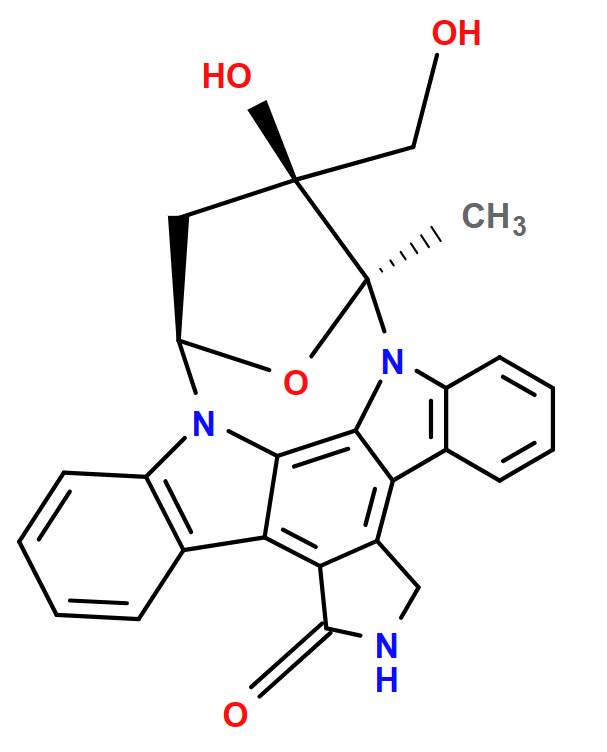
\includegraphics[width=.7\linewidth]{imagenes/estado_arte/Lestaurtinib_openbabel.png}
  \caption{OpenBabel}
  \label{fig:sub1}
\end{subfigure}%
\begin{subfigure}{.5\textwidth}
  \centering
  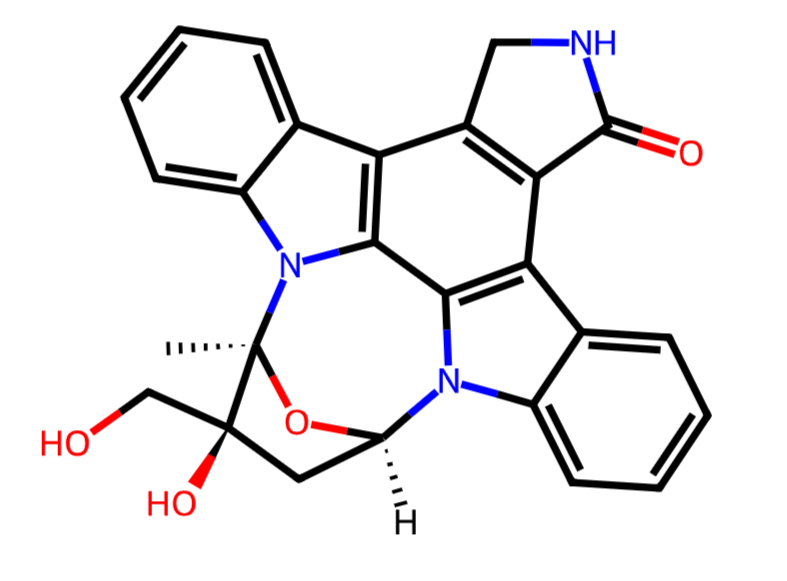
\includegraphics[width=.9\linewidth]{imagenes/estado_arte/Lestaurtinib_rdkit.png}
  \caption{RDKit}
  \label{fig:sub2}
\end{subfigure}
\caption{Representaciones 2D para el \emph{Lestaurtinib}, medicamento en estudio para el tratamiento de las leucemias agudas y algunos otros tipos de cáncer. \textbf{(a)} ha sido generado con OpenBabel; y \textbf{(b)} ha sido generado con RDKit.}
\label{fig:ejemplo_rdkit_vs_babel}
\end{figure}



OpenBabel por otro lado, ofrece más libertad en este sentido siendo capaz de leer todos los SMILES del set del que partimos. Pero en general, algo que hacen mal ambos paquetes es dibujar. Para moléculas convencionales, moléculas orgánicas o inorgánicas sencillas funciona bien, pero las organometálicas les supone un reto, y dada la escasa literatura en el tema (ver Sección \ref{revision_bib}), no dispongo de muchas referencias de las que partir.




(del archivo de informeReuniones puedo ir sacando cosas para meter en el estado del arte) Openbabel como tal no soporta el dibujado en 3D de las moléculas, por lo que los únicos dibujos que puede hacer son en 2D. Openbabel tampoco soporta el uso de wedge ni hash bonds para el dibujado de moléculas en 2D con perspectiva (es curioso porque en el código sí que hay funciones dedicadas a esto, pero luego cuando le metes símbolos SMILES de @@ y demás, los medio ignora. Sigo ejemplos del tutorial de Daylight, pero no salen los mismos dibujos. Otros símbolos más dedicados a geometría que viene en Daylight o en OpenSMILES, tipo @SP, @TB, @OH, los ignora por completo). Pero sí es capaz de generar archivos .sdf con información 3D, que se pueden usar en otros softwares de dibujado específicos como Avogadro (y no están mal, mucho mejor que los 2D desde luego)

Comparar con un ejemplo los SMILES fragmentados de SA y los completos de SF.
-	Estoy viendo que los SMILES de SA son muy malos. Prácticamente todos usan el punto, por lo que los dibujos salen separados (no es muy útil esto). SF arregla esto con el uso de ciclos, haciendo que los enlaces estén en condiciones; pero openbabel sigue haciendo los dibujos muy pegados, y superponiendo símbolos (sobre todo en compuestos que a mano se dibujarían con perspectiva. Los compuestos que son planos los dibuja bastante bien (si tiene muchos atomos quizás se solapan un poco, pero se ve bien), y aquí tampoco hay mucho margen de mejora)





\bigskip

Cuando acabe el estado del arte, tengo que dejar claro el problema que existe y que es lo que no funciona de lo que hay, para dar pie a los capítulos de desarrollo. Algo del estilo: “todo esto es lo que hay ahora (refiriéndome a lo que haya escrito arriba)” \bigskip “y tiene los siguientes problemas: blah blah” (estos problemas ya los habré mencionado seguramente en la motivación (haré referencia a ellos), pero aquí los podré extender un poco quizás); Por lo que en las siguientes secciones se dará pie a una posible solución tanto para la nomenclatura canónica como para el dibujado de las moléculas con OpenBabel.



\subsection{Herramientas de bocetado}
Simplemente para mencionarlas, herramientas tipo ChemDraw \cite{chemdraw_page} son las que los químicos e investigadores utilizan para dibujar manualmente las moléculas que luego añaden a sus publicaciones. Son este tipo de dibujos también los que probablemente podemos ver en algunas bases de datos como SigmaAldrich. En la Figura \ref{fig:chemdraw} se muestra su interfaz y algunas moléculas bocetadas.

\begin{figure}[h!]
    \centering
    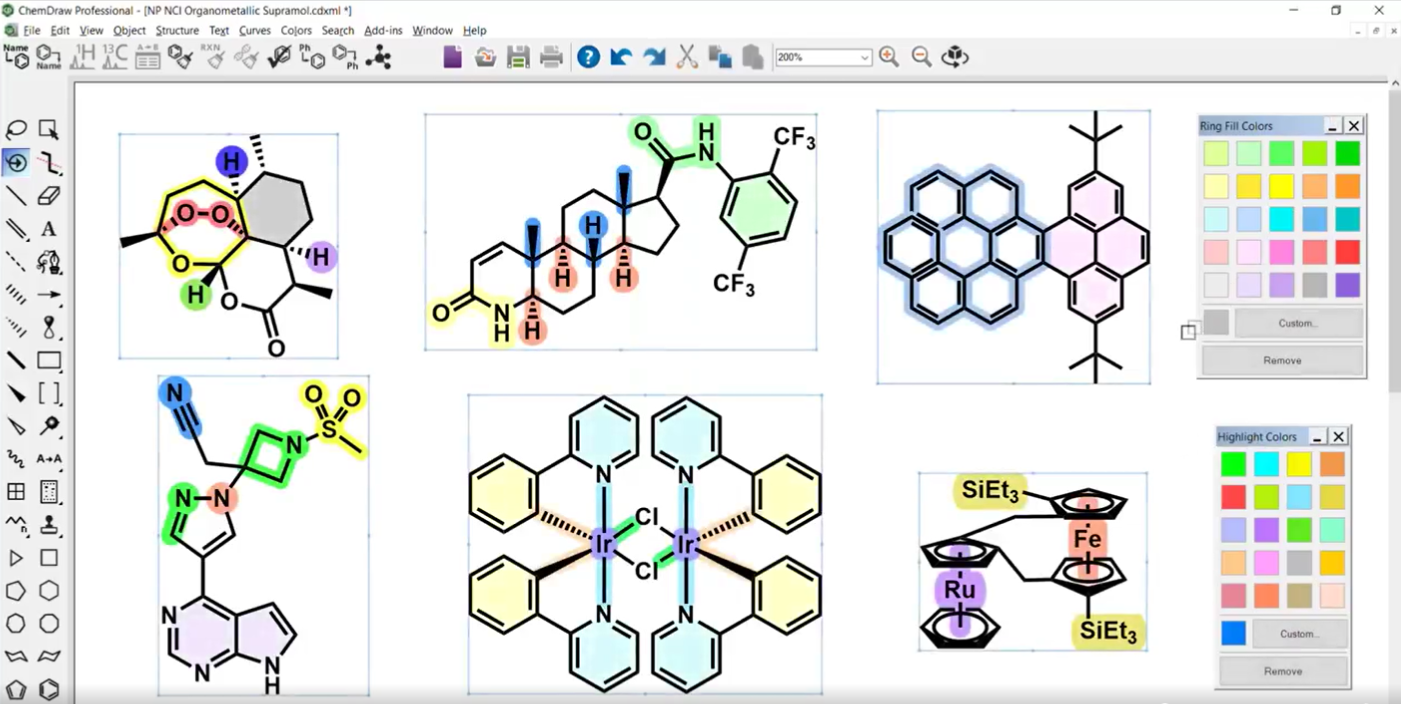
\includegraphics[scale=0.34]{imagenes/estado_arte/chemdraw.png}
    \caption{Interfaz de ChemDraw con algunas moléculas de prueba. Imagen extraída de la cuenta oficial de Facebook de ChemDraw\footnotemark}
    \label{fig:chemdraw}
\end{figure}

\footnotetext{\url{https://www.facebook.com/watch/?v=5607150085966960}}


